\chapter{Desarrollo en Robotstudio}\label{chp-06}

\lettrine[lraise=-0.1, lines=2, loversize=0.2]{L}a idea principal del proyecto es orientar el sistema para la realización de prácticas de 
laboratorio, por lo que el trabajo a realizar por los alumnos está en la programación en 
RobotStudio. Por esta razón, este capítulo va orientado a dar las pautas necesarias para el 
funcionamiento del sistema y su integración en el ecosistema de ABB. Este capítulo se basa 
en gran medida al trabajo previo de Hinojosa\cite{rea}.

\section{Funcionamiento sin microcontrolador}

El caso más simple de funcionamiento es cuando no hay microcontrolador. En este caso se
utilizarán las entradas y salidas digitales del controlador para realizar los movimientos.
La conexión entre las salidas digitales del panel de control y el controlador se realiza mediante 
un módulo de interfaz como el mostrado en la figura \ref{fig:interfazfisicadigital}.

\begin{figure}[hbtp]
    \centering
    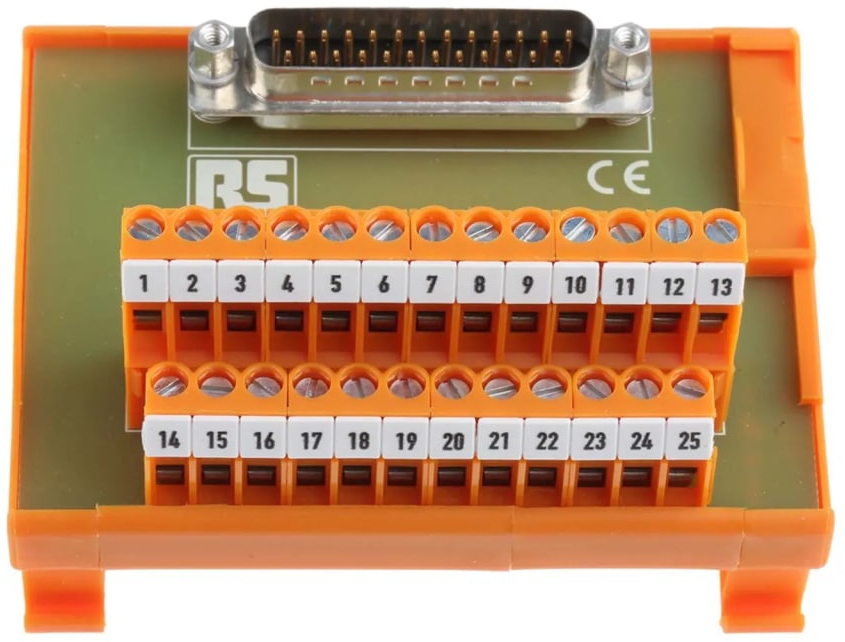
\includegraphics[width=\textwidth/2]{06-robotstudio/interfazdigital.jpg}
    \caption{Amplificación señales calibre digital a 5V}
    \label{fig:interfazfisicadigital}
    \end{figure}

Dicho módulo se conecta a la placa DSQC 652 que se encuentra montada en el controlador del robot.
Este dispositivo está diseñado para manejar señales digitales entre el sistema del robot y sistemas
como el de este proyecto. Los pines expuestos en el módulo de interfaz son los siguientes:
\begin{itemize}
    \item Entradas (DI, Digital Inputs). Pines del 1 al 8 que corresponden a los DI01 a DI08.
    \item Salidas (DO, Digital Outputs). Pines del 14 al 24 que corresponden a los DO01 a DO08.
    \item GND. Pin 24.
    \item VCC 24V. Pin 25.
\end{itemize}

En éste, los pines de salida se conectarán a las señales de Avance y Retroceso, mientras que en los de entrada estarán la señal del sensor fotoeléctrico, la de emergencia, el estado de la señal local y la señal microcontrolador.

Las funciones referentes a las señales digitales se pueden consultar en el manual de RAPID \cite{rapid}.
Las más relevantes para el uso básico requerido en el laboratorio:
\begin{itemize}
    \item SetDO, cambio de valor en salida digital. Uso: SetDo señalDO, valor;
    \item Lectura de entrada digital. Se puede realizar simpelmente utilizando el nombre de la señal. 
    Usos: estado-actual := señalDI; IF señalDI = valor DO ...
    \item WaitDI, espera en el programa hasta que una señal de entrada tome cierto valor.
    Uso: WaitDI señalDI, valor;
\end{itemize}

Un ejemplo de programa es el que se puede ver en el código \ref{no_micro}. Este programa consiste en hacer avanzar
la cinta hasta que se enciende el sensor fotoeléctrico.
Una vez detecta esa señal, el robot recoge la pieza y se repite la operación 
haciéndolo retroceder. Para ello, se debe definir el \textit{workobject} de la cinta transportadora para mover
el brazo robótico sobre sus ejes. Posteriormenete se debe definir la posición de recogida del brazo donde 
se activa el sensor fotoeléctrico. Las demás posiciones se generarán mediante \emph{offsets} de la posición de recogida.
El trabajo con el brazo robótico queda a cargo de futuros alumnos, aquí se muestra exclusivamente el trato 
con las señales digitales. Para simplificar los nombres de las señales se utilizan nombres descriptivos, no
el que realmente aparece en RobotStudio.

\begin{lstlisting}[language=,caption={Ejemplo de programa sin microcontrolador}, breaklines=true, label=no_micro]
MODULE Module1
    !Aquí deben estar definidas las posiciones y variables auxiliares
    !
    PROC main()
        !Se procede a avanzar 
        SetDO señalAvance, 1;
        SetDO señalRetroceso, 0;

        !Se espera a que se active el sensor fotoeléctrico
        WaitDI señalFoto, 1;
        !Se para la cinta
        SetDO señalAvance, 0;
        SetDO señalRetroceso, 0;
        
        !Movimiento del brazo robótico para recoger la pieza y colocarla en una posición avanzada donde haya que retroceder
        ...

        !Misma operación a la inversa
        SetDO señalAvance, 0;
        SetDO señalRetroceso, 1;

        !Se espera a que se active el sensor fotoeléctrico
        WaitDI señalFoto, 1;
        !Se para la cinta
        SetDO señalAvance, 0;
        SetDO señalRetroceso, 0;

        !Movimiento del brazo robótico para recoger la pieza y colocarla en la posición original
        ...
    ENDPROC
END MODULE
\end{lstlisting}
    

\section{Funcionamiento con microcontrolador}

El funcionamiento del sistema con microcontrolador permite al controlador del robot tener la información
completa sobre la posición de la pieza a lo largo de la cinta y del estado del sistema. Para poder 
transmitir los datos se realizará una conexión TCP/IP donde Arduino y controladora se enviarán
información mutuamente. Para que esta opción esté habilitada en RobotStudio, es necesario añadir la 
funcionalidad "PC Interface" durante la creación de la estación. El procedimiento para realizar la conexión 
y el envío de datos se encuentra explicado demostrado en Hinojosa\cite{rea}, mientras que en el código 
\ref{cod_micro} se encuentra un ejemplo funcional.

La comunicación es bidireccional: la controladora del robot envía una orden mientras que el Arduino responde
en consecuencia. Existen tres órdenes enviadas por la controladora diferentes:
\begin{itemize}
    \item Solicitud de posición y estado, se envía la cadena "STATUS" al Arduino.
    \item Orden de movimiento absoluto. Se envía una cadena con el carácter "M" seguido de la posición final en 
    milímetros con el formato ";X=" + posición.
    \item Orden de avance discreto. Se envía una cadena con el carácter "R" seguido de los milímetros que tiene
    que avanzar la cinta con el formato ";X=" + avance.
\end{itemize}

En el caso de recibir una cadena "STATUS", el Arduino responderá con una cadena con el siguiente formato:

Carácter de estado + ";X=" + posición + ";Y=" medida del calibre + ";F=" + valor del sensor fotoeléctrico.

El microcontrolador del Arduino está continuamente comprobando si existe una orden por parte de la controladora,
ya que se comprueba en muchas partes del código, independientemente de si se encuentra en modo local o en modo
remoto. Sin embargo, si se encuentra en modo local únicamente responderá a la solicitud de "STATUS", ya que 
no puede recibir órdenes de movimiento en este modo. En modo remoto, si recibe una orden de movimiento, pasará
automáticamente al estado de movimiento con los datos recogidos y realizará dicho movimiento.

A continuación se incluye el código \ref{cod_micro} necesario para la lectura del estado y la posición, además del envío
de movimiento absoluto y discreto.

\begin{lstlisting}[language=,caption={Ejemplo de programa con microcontrolador}, breaklines=true, label=cod_micro]
MODULE Module1  
    !Declaración de variables del programa
    !Objeto de socket de conexión
    VAR socketdev my_socket;

    !Variable de estado
    VAR string estado:=0;

    !Cadenas de caracteres de recepción
    VAR rawbytes receive_string;
    VAR string string1;
    VAR string posx_str;
    VAR string posy_str;
    VAR string fotoele_str;

    !Posiciones de los datos a lo largo de la cadena recibida
    VAR num xpos;
    VAR num ypos;
    VAR num fepos;
    
    !Valores numéricos finales recibidos
    VAR num posx;
    VAR num posy;
    VAR byte fotoele;
    
    !Comprobación de recepción correcta
    VAR bool okposx:=true;
    VAR bool okposy:=true;

    !Bucle principal del programa
    PROC main()
        !Se cierran los posibles sockets abiertos
        SocketClose my_socket;
        
        WaitTime 0.2;
        
        !Función de lectura de posición y estado
        leer;

        !Movimiento absoluto
        mov_abs(200);

        !Movimiento discreto
        mov_dis(100);

        WaitTime 0.5;
    ENDPROC
    
    !Función de apertura de socket
    PROC abricomunicacion()        
        SocketCreate my_socket; !crea el socket
        SocketConnect my_socket, "192.168.50.200", 4012;        
    ENDPROC
    
    !Función de lectura de estado y 
    PROC leer()
        !Se abre el socket y conecta al Arduino
        abricomunicacion;
        
        !Escribe en el socket la cadena "STATUS" para que el Arduino envíe sus datos
        SocketSend my_socket,\Str:="STATUS"; 
        WaitTime 0.1; !espera un tiempo

        !Recibe la respuesta 
        ClearRawBytes receive_string;
        SocketReceive my_socket \RawData := receive_string,\Time:=WAIT_MAX;
        
        !Desempaqueta los bytes y los convierte en una cadena de caracteres
        UnpackRawBytes receive_string, 1, string1 \ASCII:=32;
        
        !Se buscan las posiciones de cada variable a lo largo de la cadena
        xpos        := StrFind(string1, 1, "=");
        ypos        := StrFind(string1, xpos+1, "=");
        fepos       := StrFind(string1, ypos+1, "=");
        
        !Se trocea la cadena para obtener subcadenas con los datos recibidos
        estado      := StrPart(string1, 0, 1);
        posx_str    := StrPart(string1, xpos+1, ypos - xpos - 3);
        posy_str    := StrPart(string1, ypos+1, fepos - ypos - 3);
        fotoele_str := StrPart(string1, fepos+1, 1);

        !Se transforman las cadenas a los tipos de datos que les corresponden
        okposx      :=  StrToVal(posx_str,posx);
        okposy      :=  StrToVal(posy_str,posy);
        fotoele     :=  StrToByte(fotoele_str);
        
        !Conversión de pulsos a milímetros
        posx := posx / 100;

        !Se cierra el socket
        ClearRawBytes receive_string;
        SocketClose my_socket;
    ENDPROC

    !Funciones de movimiento. Se envía una cadena con un caracter y la distancia a recorrer. Si el carácter es "M", el movimiento es absoluto, mientras que si es "R" es relativo.
    PROC mov_abs(num distancia)
        abricomunicacion;
        SocketSend my_socket,\Str:="M;X=" + ValToStr(distancia*100) + ";";
        WaitTime 0.1;
        SocketClose my_socket;
    ENDPROC
    
    PROC mov_dis(num distancia)
        abricomunicacion;
        SocketSend my_socket,\Str:="R;X=" + ValToStr(distancia*100) + ";";
        WaitTime 0.1;
        SocketClose my_socket;
    ENDPROC
ENDMODULE
\end{lstlisting}
    

Una vez obtenida la posición de la pieza en los ejes x e y, hay que tener en cuenta que dicha posición está expresada en unos ejes concretos definidos desde el comienzo de la cinta. Por ello, hay que crear 
un \emph{workobject} en el proyecto de Robotstudio donde estos ejes tengan la misma dirección que los ejes de la cinta para, posteriormente poder transformar las posiciones obtenidas por parte del Arduino a unas unidades utilizables por parte del robot y del propio usuario.